\documentclass[10pt]{article}
\usepackage{tikz}
\usetikzlibrary{shapes.misc}
\usepackage[margin=0cm]{geometry}
\pagestyle{empty}
\tikzstyle{every node}=[cross out, draw, red]

\begin{document}

\vspace*{\fill}
\begin{center}
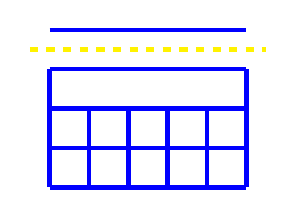
\begin{tikzpicture}[x=0.5cm, y=-0.5cm, ultra thick, blue]
% Walls
    \draw (0,0) -- (5,0);
    \draw (0,1) -- (5,1);
    \draw (0,2) -- (5,2);
    \draw (0,3) -- (5,3);
    \draw (0,4) -- (5,4);
    \draw (0,1) -- (0,4);
    \draw (1,2) -- (1,4);
    \draw (2,2) -- (2,4);
    \draw (3,2) -- (3,4);
    \draw (4,2) -- (4,4);
    \draw (5,1) -- (5,4);
%Pillars
%Inner points in accessible cul-de-sacs
%Entry-exit paths without intersections
    \draw[dashed, yellow] (-0.5,0.5) -- (5.5,0.5);
\end{tikzpicture}
\end{center}
\vspace*{\fill}

\end{document}
